% What does this text have to do with the oracular query that this
% section introduces???  You have to explain the most salient features
% of the section -- like the title -- before diving into details!  -Scott
%
% The main complaint about patent search is an
% insufficient match between the content of patent queries and
% relevant
% patents\cite{lupu2013patent}\cite{magdy2012toward}. However,
% considering the size of a patent query (usually thousand of words),
% the intuition is that there are enough terms to match the relevant
% patents.

In this section we develop an \emph{Oracular Query} to understand (a)
the adequacy of the baseline
\emph{Patent Query}, (b) an upper bound on performance of the
BM25 and LM models, and (c) the sufficiency of terms in the reference
patent query.

\subsection{Oracular Query Formulation}

% As noted previously, I would be careful calling this ``relevance feedback''
% and especially abbreviating it RF since RF usually has a different definition
% based on a vector space or other model.  I would call it AvgRelDiff or
% something similar.  -Scott
We begin by defining an oracular relevance feedback system, which
extracts terms from the judged relevant documents. To this end, after an initial run of a given query, we
calculate a Relevance Feedback ($\mathit{RF}$) score for each term $t$ in the top-100
retrieved documents for query $Q$ as follows:
% Use \mathit{RF}, \mathit{Rel}, etc. for multiletter names, 
% otherwise RF is technically R*F!  Fix.  -Scott
\begin{equation}
RF(t,Q)=Rel(t,Q)-Irr(t,Q) 
 \label{eq:score}
\end{equation}\vspace*{-5ex}
\begin{displaymath}t\in \lbrace \mbox{terms in top-100 retrieved documents}\rbrace\end{displaymath}
where $ \mathit{Rel(t,Q)} $ is the \textcolor{black}{average term frequency} in retrieved relevant patents and $ \mathit{Irr(t,Q)} $ is the average term frequency in retrieved irrelevant patents. We assume that words with a positive score are \emph{useful words} since they are more frequent in relevant patents, while words with negative score are \emph{noisy words} as they appear more frequently in irrelevant patents. We empirically seek to evaluate the threshold $\tau$ on $RF(t,Q)$ (defined below) yielding the best oracular query.

%that determines if a term is selected to build the \emph{Oracular Query} or not.

% Huh??? -Scott
%
%We expected to see a higher performance for the queries which contain more \textit{ useful words}, but, surprisingly, we could not find any correlation between the performance and the presence of \textit{ useful words} in the query. 

%We hypothesized that a query, formulated by only the \textit{ useful terms}, is the best possible query we can make since they are all frequent in relevant patents but rare in irrelevant ones. 
We formulate two oracular queries. The first query is formulated by selecting terms in the top-100 documents:
\begin{equation}
Oracular \; Query = \{t \in \textrm{top-100}|RF(t, Q)>\tau\}   
 \label{eq:score}
\end{equation}
We formulate the second query by selecting terms that also occur in the reference patent query as follows:
% query based on the hypothesis that a patent query contains sufficient words matched with the relevant patents:
\begin{equation}
 Oracular \; Patent \; Query = \{t\in Q|RF(t, Q)>\tau\}   
 \label{eq:score}
\end{equation}
%The system performance to these two queries were encouraging. We discuss the detailed results in the next section.

\subsection{Baseline vs. Oracular Query}

\label{sec:baseline_vs_oracular}

%%%%%%%%%%%%%%%%%%%%%%%%%%%%%%%%%%%%%%%%%%%%%%%%%%%%%%%%%%%%%%
\begin{figure}[t!]
\begin{centering}
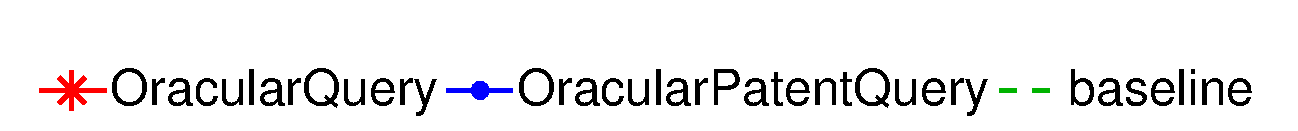
\includegraphics[width=9cm]{imgs/l1}
\par\end{centering}

\begin{centering}
\subfigure[{Mean Average Precision.}]{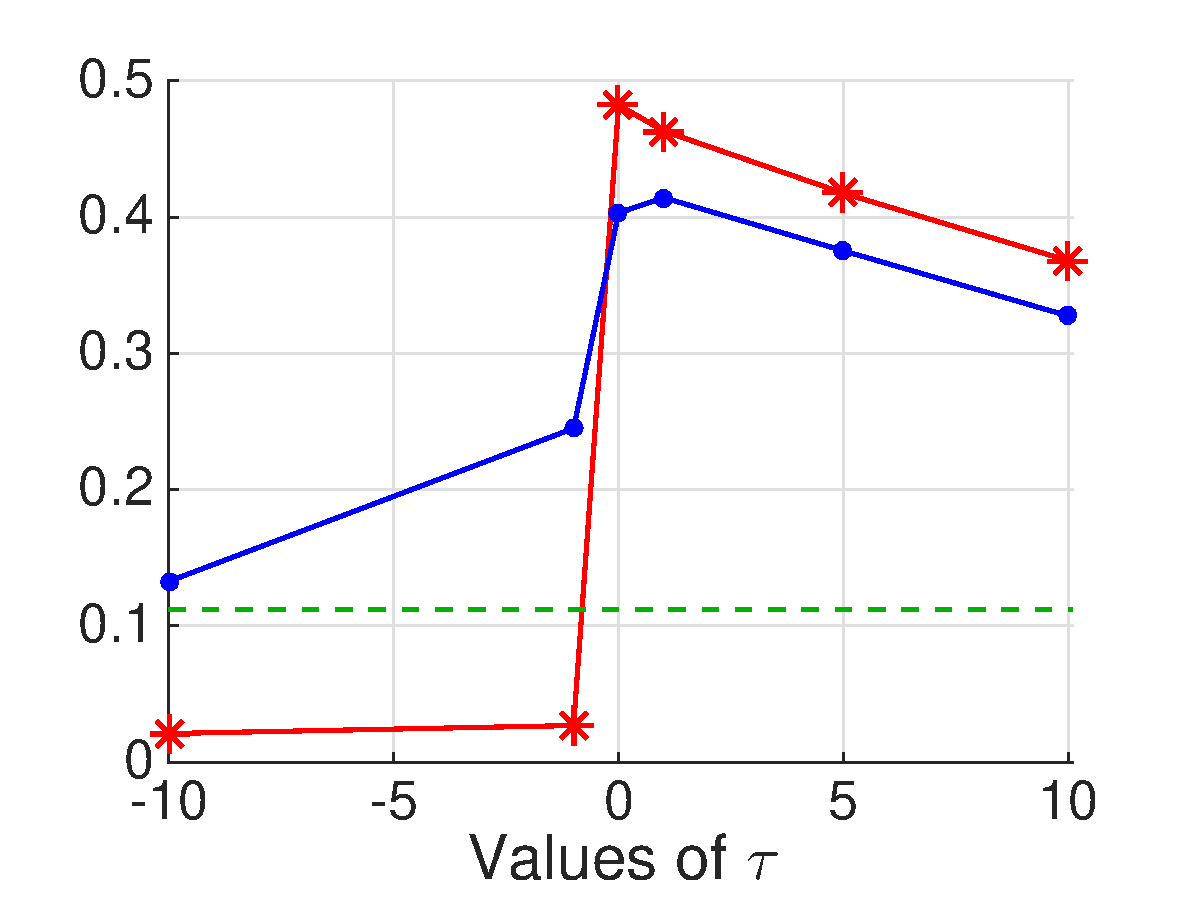
\includegraphics[width=4.5cm]{imgs/fig1_map_cr}}\subfigure[Recall.]{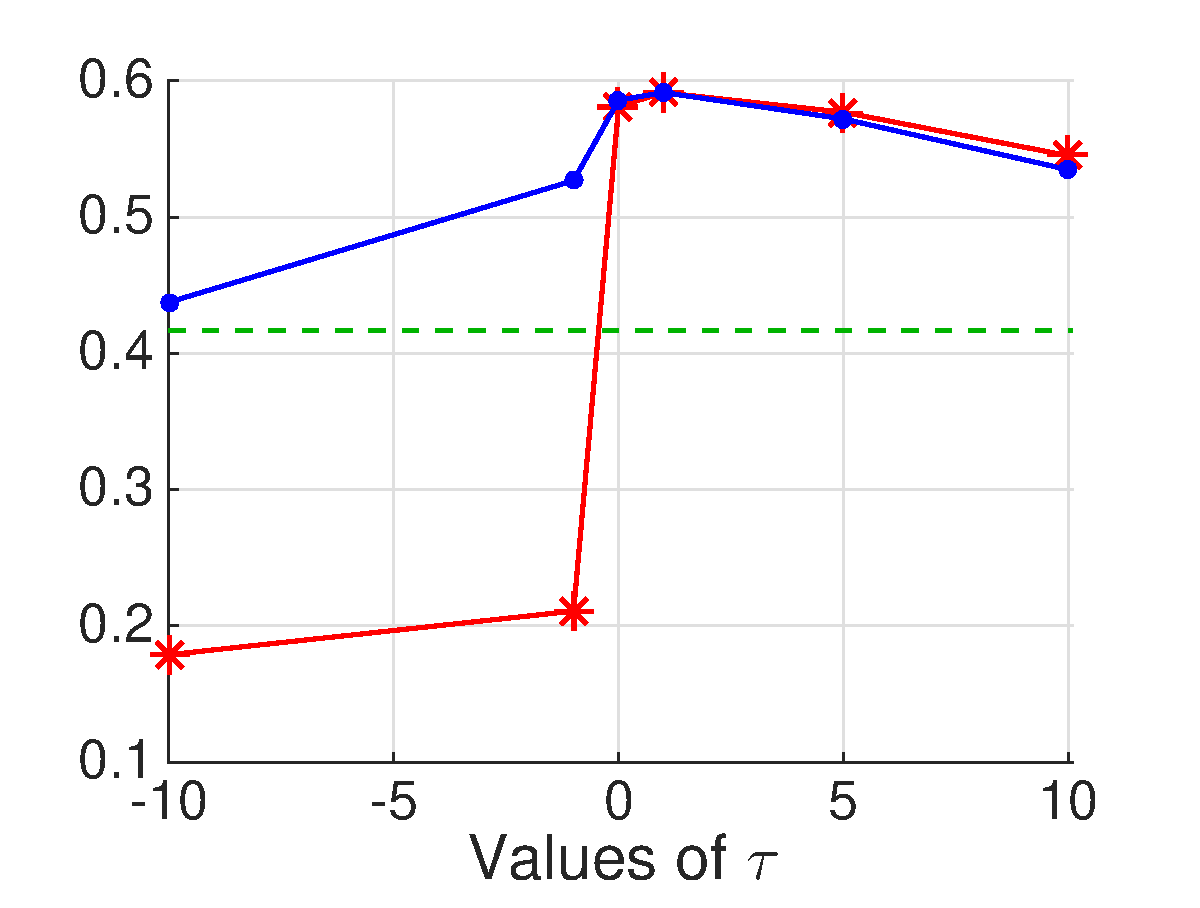
\includegraphics[width=4.5cm]{imgs/fig1_recall_cr}}
\par\end{centering}

\protect\caption{System performance vs. the threshold $\tau$ for Oracular Query and Oracular Patent Query.}
\label{fig:oracular}
\end{figure}
%%%%%%%%%%%%%%%%%%%%%%%%%%%%%%%%%%%%%%%%%%%%%%%%%%%%%%%%%%%%%%

% Scott: for clarity, the discussion now proceeds from low tau to middle
%        tau to high tau.  Discussion of PATATRAS comes once Table 1 has
%        been discussed.
First, we investigate the ideal threshold setting $\tau$ for the
oracular queries as shown in Figure \ref{fig:oracular}.  Notably,
there is a rather unexpected steep drop-off in performance for both
oracular queries when slightly noisy terms are included
(i.e., $\tau$ just slightly less than 0).  However, this dropoff is
less pronounced for the
\emph{Oracular Patent Query} indicating that restriction to query terms in the
reference patent may reduce the impact of the noisy terms that are present.
While the \emph{Oracular Query} and \emph{Oracular Patent Query} peak
at slightly different thresholds ($\tau = 0$ and $\tau = 1$, respectively), 
either value of $\tau$ yields good performance.
However, values of $\tau > 1$
demonstrate a stronger relative decrease in performance due to the exclusion 
of a large number of useful terms.

% Scott: While true, I don't think this adds much insight... I tried
%        to provide more insight in the edits above.
%MAP begins to improve over the baseline when we prune noisy words out of the \emph{Patent Query} by increasing the value of $\tau$; it approaches its highest value at $\tau=1$, where it starts decreasing due to loss of useful words.

% What is the ``Best Run''???  You cannot make up words and expect the
% reader to understand.  Be precise on the first introduction that
% this is the best result from CLEF-IP 2010 and provide a citation.
% And call it the ``Top CLEF-IP 2010'' system to be crystal clear.
% Furthermore, it has been mentioned previously that the MAP from CLEF-IP 2010
% and the MAP you provide are not directly comparable since some topics are
% excluded from this evaluation --- for full disclosure you need to explain
% all details of how these MAP measurements differ (and hence indicate this
% Top CLEF-IP 2010 result is only included for a rough comparison of
% performance).  Fix all of these issues and all name changes resulting
% from these updates.  -Scott
%
% Update this discussion with the new table contents.  -Scott
%
% Also, streamline the text... so many sentences are redundant or 
% unneccessary!  You're not done writing until you've removed every
% word possible without changing the meaning of what's written.  -Scott
%
% If different \tau's were used then be clear on this, or simply mention
% Oracular Patent Query $\tau=1$ in the table entry and mention in the
% text how this optimal \tau was selected.  Maybe Figure 1 should come
% before Table 1?  This would better explain how the best \tau's were
% selected.  -Scott
%

%%%%%%%%%%%%%%%%%%%%%%%%%%%%%%%%%%%%%%%%%%%%%%%%%%%%%%%%%%%%%%
\begin{table}[t!]
  \vspace{-1mm}
  \begin{center}
  \scriptsize
   \caption{Performance for the \textit{ Patent Query} (baseline), two variants of the \textit{ Oracular Query}, and \textit{ Top CLEF-IP 2010 Competitor (PATATRAS)}.}
   \vspace*{1ex}
  \input table/table1-cr.tex   
  \label{tab:optquery}
  \end{center}  
\vspace{-3mm}
\end{table}
%%%%%%%%%%%%%%%%%%%%%%%%%%%%%%%%%%%%%%%%%%%%%%%%%%%%%%%%%%%%%%
%%%%%%%%%%%%%%%%%%%%%%%%%%%%%%%%%%%%%%%%%%%%%%%%%%%%%%%%%%%%%%
%\begin{table}[t!]
%  \begin{center}
%  \scriptsize
%   \caption{\textcolor{red}{NOT-FILTERED} Performance for the \textit{ Patent Query}, two variants of the \textit{ Oracular Query}, and \textit{ Top CLEF-IP 2010 (PATATRAS)}.}
%   \vspace*{1ex}
%  \input table/optquery-actual.tex   
%  \label{tab:optquery}
%  \end{center}  
%\end{table}
%%%%%%%%%%%%%%%%%%%%%%%%%%%%%%%%%%%%%%%%%%%%%%%%%%%%%%%%%%%%%%

In Table~\ref{tab:optquery}, we compare our best oracular relevance
queries with both the baseline \textit{Patent Query} and the PATATRAS
system.  In general we found BM25 and LM to offer very similar
performance.  Our subsequent results use only LM due to space
limitations although results for BM25 are very similar.  More
importantly, the \emph{Oracular Query} using $\tau=0$ far
outperforms the baseline and approximately performs twice as well on
MAP as the PATATRAS system, the best competitor in CLEF-IP 2010.  The
MAP and the recall for the best \emph{Oracular Patent Query} are
respectively lower than the MAP and the recall for the
best \emph{Oracular Query}.  However, the query reduction approach
inherent in the \emph{Oracular Patent Query} is still sufficient to
achieve MAP performance appreciably better than PATATRAS (for
$\tau \geq 0$) with reduced sensitivity to the inclusion of noisy
terms (when $\tau < 0$).

%selecting terms from the reference
%patent query itself (for $\tau \geq 0$) are still sufficient to achieve
%MAP performance appreciably better than PATATRAS with reduced sensitivity
%to the inclusion of noisy terms (when $\tau < 0$).

%
% Unweighted is most natural so no need to even mention it.  -Scott
%
%We observed that a weighed --by query term
%frequency-- query performs better than the unweighed one. However, our
%oracular query performed better unweighed, so, we compare the results
%with unweighed baseline query. The \textit{ best run} in CLEF-IP 2010
%achieved 0.27 MAP~\cite{lopez2010experiments}.

%Next, we used a threshold $\tau$ to formulate the \textit{ Oracular Query}
%and \textit{ Oracular Patent Query} to include merely terms with the RF
%score higher than $\tau$ ($RF(t,Q)>0$).

% Good: is space allows, the enumeration helps make the take-home points
% of this section clear for the reader and leads into the next section.  -Scott

Hence, our experiments related to oracular relevance feedback system
suggest two important conclusions: (1) query reduction should suffice for effective prior art patent retrieval; and (2) very precise methods for eliminating poor query terms in the reduction process are needed.


